% Five-minute NeurIPS 2026 talk: Tokens-per-Parameter Coverage Is Critical for Robust LLM Scaling Law Extrapolation.
% Build: make (from this folder). Logos come from ../images (SVG, converted by the Makefile); figures from figures/.
\documentclass[aspectratio=169,11pt]{beamer}
\usetheme{default}
\usecolortheme{default}
\setbeamertemplate{navigation symbols}{}
\setbeamertemplate{footline}[frame number]
\setbeamercolor{frametitle}{fg=black}
\setbeamercolor{structure}{fg=orange!80!black}
\setbeamertemplate{itemize items}[circle]
\usepackage{amsmath,amssymb,booktabs,tikz,graphicx}
\usetikzlibrary{arrows.meta}
\graphicspath{{figures/}{build/}}
% Short author-year sources, set at the foot of the slide that uses them.
\newcommand{\slidecite}[1]{\vfill{\tiny\color{gray}#1\par}}

\title{Tokens-per-Parameter Coverage Is Critical for\\Robust LLM Scaling Law Extrapolation}
\author{Joshua Shay Kricheli\textsuperscript{*}\quad Alexander Lawrence Reid\textsuperscript{*}\quad
  Soumajyoti Sarkar\\ Venkata Gandikota\quad Paulo Shakarian}
\institute{Syracuse University: Leibniz Lab, Institute for Artificial Intelligence\quad
  Amazon AGI Foundations\textsuperscript{\dag}\\[2pt]
  {\scriptsize \textsuperscript{*}Equal contribution.\quad
  \textsuperscript{\dag}This work does not relate to the author's position at Amazon.}}
\date{NeurIPS 2026, Sydney}

\begin{document}

\begin{frame}[plain]
  \titlepage
  \vspace{-6pt}
  \centering
  \includegraphics[height=0.6cm]{neurips.pdf}\hspace{0.5cm}%
  \includegraphics[height=0.6cm]{syracuse_university.pdf}\hspace{0.5cm}%
  \includegraphics[height=0.6cm]{syracuse_ai_institute.pdf}\hspace{0.5cm}%
  
\includegraphics[height=0.6cm]{../images/leibniz_lab.png}
\end{frame}

\begin{frame}{Motivation and collinear designs}
  \begin{columns}[c]
    \begin{column}{0.52\textwidth}
      \begin{itemize}\setlength{\itemsep}{6pt}
        \item Motivation: LLM runs cost millions; labs fit scaling laws [1,~2] to choose $N$, $D$, not trial and~error
        \item Chinchilla rule: $k = D/N \approx 20$ tokens per parameter [1]; often one fixed $k$, one~ray
        \item Chinchilla law [1], on a ray both terms move~together:\\[4pt]
          $L(N, kN) = A N^{-\alpha} + B k^{-\beta} N^{-\beta} + E$
        \item Only the gap $\varepsilon = |\alpha - \beta|$ separates $A$ from~$B$
      \end{itemize}
    \end{column}
    \begin{column}{0.44\textwidth}
      \centering
      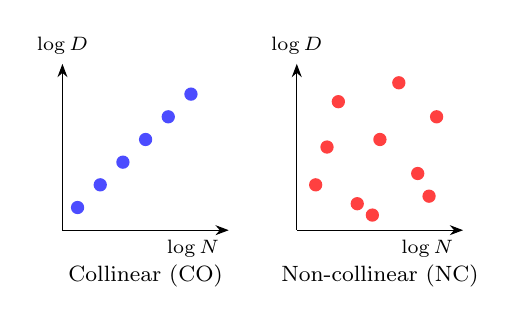
\begin{tikzpicture}[scale=0.48]
        \foreach \x/\lab in {0/Collinear (CO), 6.2/Non-collinear (NC)} {
          \draw[-{Stealth}] (\x,0) -- (\x+4.4,0) node[below left] {\scriptsize $\log N$};
          \draw[-{Stealth}] (\x,0) -- (\x,4.4) node[above] {\scriptsize $\log D$};
          \node at (\x+2.2,-1.2) {\footnotesize \lab};
        }
        \foreach \i in {0,...,5} {
          \fill[blue!70] (0.4+0.6*\i, 0.6+0.6*\i) circle (5pt);
        }
        \foreach \i/\j in {0.5/1.2, 1.1/3.4, 1.6/0.7, 2.2/2.4, 2.7/3.9, 3.2/1.5, 3.7/3.0, 0.8/2.2, 2.0/0.4, 3.5/0.9} {
          \fill[red!75] (6.2+\i, \j) circle (5pt);
        }
      \end{tikzpicture}
    \end{column}
  \end{columns}
  \slidecite{[1] Hoffmann et al., NeurIPS 2022.\quad [2] Kaplan et al., arXiv 2020.}
\end{frame}

\begin{frame}{Theory: when the scale pair is identified}
  \begin{itemize}
    \item One ray: $\kappa_{A,B} = \Theta(\varepsilon^{-2})$; CI on $A$ is $\Omega(\varepsilon^{-1})\times$ CI on $\psi = A + Bk^{-\alpha}$
    \item $K$ rays: $\kappa_{A,B} \leq \kappa_{\mathrm{target}}$ (leading order) whenever
  \end{itemize}
  {\small\[
    \underbrace{\frac{1}{K}\sum_{\ell=1}^{K} k_\ell^{-2\beta_{\mathrm{eff}}}
      - \Bigl(\frac{1}{K}\sum_{\ell=1}^{K} k_\ell^{-\beta_{\mathrm{eff}}}\Bigr)^{2}}_{V_K}
    \;\geq\;
    \underbrace{\frac{\bigl(K + \sum_{\ell} k_\ell^{-2\beta_{\mathrm{eff}}}\bigr)^{2}}{K^{2}\,\kappa_{\mathrm{target}}}}_{\tau_K},
  \]}
  \begin{itemize}
    \item Exact: $\kappa_{A,B} \leq \kappa_{\mathrm{target}}$ iff $V_K \geq \tau_K/(1 + 1/\kappa_{\mathrm{target}})^2$
    \item One ray never passes; two pass once $k_2/k_1 \geq R_{\min}(k_1)$
    \item Checkable before~training
  \end{itemize}
\end{frame}

\begin{frame}{Results: non-collinear designs extrapolate}
  \begin{columns}[T]
    \begin{column}{0.51\textwidth}
      \small
      \begin{tabular}{@{}lr@{}}
        \toprule
        Comparison (NC vs.\ CO) & NC wins \\
        \midrule
        Full fan, FP32 (1,460 of 1,500) & $97.3\%$ \\
        Full fan, BF16 (296 of 300) & $98.7\%$ \\
        \midrule
        Budget-matched, Chinchilla [1] & $68.5\%$ \\
        Budget-matched, Droppo-Elibol [3] & $57.4\%$ \\
        Budget-matched, Kaplan [2] & $80.6\%$ \\
        \bottomrule
      \end{tabular}

      \vspace{6pt}
      \begin{itemize}
        \item 1,900 models, 5M-77M params
        \item 5 corpora; 4 laws [1-4]
        \item Budget-matched: CO subsets below~threshold
      \end{itemize}
    \end{column}
    \begin{column}{0.45\textwidth}
      \centering
      \includegraphics[width=0.85\linewidth]{01_convergence_Red_Pajama_Kaplan_First.pdf}\\
      {\scriptsize Holdout $R^2$ against TPP coverage (Kaplan, RedPajama).}
    \end{column}
  \end{columns}
  \slidecite{[1] Hoffmann et al., NeurIPS 2022.\quad [2] Kaplan et al., arXiv 2020.\quad [3] Droppo and Elibol, Interspeech 2021.\quad [4] Muennighoff et al., Scaling data-constrained language models, JMLR 2025.}
\end{frame}

\begin{frame}{Takeaway and design recipe}
  \begin{columns}[T]
    \begin{column}{0.62\textwidth}
      \begin{itemize}
        \item Fit on designs that span TPP~ratios
        \item Recipe: pick $k_1$, read $R_{\min}(k_1)$, train both ends, split runs~evenly
        \item Check exact $\kappa_{A,B}$ before~training
        \item Code, data, checkpoints:~public
      \end{itemize}
      \vspace{2pt}
      \centering
      \href{https://lab-v2.github.io/tpp-coverage/}{\texttt{lab-v2.github.io/tpp-coverage}}
    \end{column}
    \begin{column}{0.34\textwidth}
      \centering
      \includegraphics[width=0.9\linewidth]{qr_project_page.pdf}
    \end{column}
  \end{columns}
\end{frame}

\end{document}
